\documentclass[a4paper,11pt]{article}

\usepackage[utf8]{inputenc}
\usepackage[T1]{fontenc}
\usepackage{graphicx}
\usepackage{hyperref}
\usepackage{xcolor}
\usepackage{tcolorbox}
\usepackage{enumitem}
\usepackage{geometry}
\usepackage{fancyhdr}
\usepackage[table]{xcolor}
\usepackage{booktabs}
\usepackage{array}
\usepackage{tabularx}
\usepackage{listings}
\usepackage{fancyvrb}
\usepackage{multicol}

\geometry{margin=2cm, top=2.5cm, bottom=2.5cm}
\setlength{\headheight}{14pt}

\definecolor{titlecolor}{RGB}{0, 90, 160}
\definecolor{sectitlecolor}{RGB}{5, 100, 175}
\definecolor{subsectitlecolor}{RGB}{10, 110, 190}
\definecolor{definitionbg}{RGB}{240, 248, 255}
\definecolor{examplebg}{RGB}{245, 255, 245}
\definecolor{warningbg}{RGB}{255, 245, 245}
\definecolor{benefitbg}{RGB}{255, 253, 235}
\definecolor{codecolor}{RGB}{240, 240, 240}
\definecolor{codekeyword}{RGB}{0, 0, 128}
\definecolor{codestring}{RGB}{163, 21, 21}
\definecolor{codecomment}{RGB}{0, 128, 0}
\definecolor{todobg}{RGB}{255, 235, 235}
\definecolor{collabg}{RGB}{245, 240, 255}

\lstset{
  basicstyle=\ttfamily\footnotesize,
  backgroundcolor=\color{codecolor},
  keywordstyle=\color{codekeyword}\bfseries,
  stringstyle=\color{codestring},
  commentstyle=\color{codecomment}\itshape,
  breaklines=true,
  showstringspaces=false,
  frame=single,
  tabsize=2,
  captionpos=b
}

\pagestyle{fancy}
\fancyhf{}
\fancyhead[L]{\textit{Lab 3 --- Le monolithe modulaire}}
\fancyhead[R]{\textit{Architectures Logicielles}}
\fancyfoot[C]{\thepage}
\fancyfoot[L]{\textit{Dr. El Hadji Bassirou TOURE}}
\fancyfoot[R]{\textit{DMI/FST/UCAD}}
\renewcommand{\headrulewidth}{0.4pt}
\renewcommand{\footrulewidth}{0.4pt}

\newtcolorbox{concept}{
  colback=definitionbg, colframe=sectitlecolor,
  title=Concept fondamental, fonttitle=\bfseries
}
\newtcolorbox{intuition}{
  colback=examplebg, colframe=green!75!black,
  title=Intuition, fonttitle=\bfseries
}
\newtcolorbox{exemple}{
  colback=orange!5!white, colframe=orange!75!black,
  title=Exemple, fonttitle=\bfseries, fontupper=\footnotesize
}
\newtcolorbox{pointcle}{
  colback=benefitbg, colframe=orange!70!black,
  title=Point cle a retenir, fonttitle=\bfseries
}
\newtcolorbox{warningbox}{
  colback=warningbg, colframe=red!70!black,
  title=Point d'attention, fonttitle=\bfseries
}
\newtcolorbox{benefitbox}{
  colback=benefitbg, colframe=green!70!black,
  title=Benefice, fonttitle=\bfseries
}
\newtcolorbox{todobox}{
  colback=todobg, colframe=red!60!black,
  title=Tache a realiser, fonttitle=\bfseries\scriptsize, fontupper=\small
}
\newtcolorbox{collabox}{
  colback=collabg, colframe=violet!70!black,
  title=Qui pilote cette section ?, fonttitle=\bfseries\scriptsize, fontupper=\small
}
\newtcolorbox{tagbox}{
  colback=yellow!15, colframe=yellow!50!black,
  title=Jalon Git, fonttitle=\bfseries\scriptsize, fontupper=\small
}

\lstset{
  basicstyle=\tiny\ttfamily,
  keywordstyle=\tiny\ttfamily\bfseries\color{codekeyword},
  commentstyle=\tiny\ttfamily\itshape\color{codecomment},
  stringstyle=\tiny\ttfamily\color{codestring}
}

\usepackage[explicit]{titlesec}
\titleformat{\section}
  {\Large\bfseries\color{titlecolor}}{\thesection}{0.5em}{#1}
\titleformat{\subsection}
  {\large\bfseries\color{sectitlecolor}}{\thesubsection}{0.5em}{#1}
\titleformat{\subsubsection}
  {\normalsize\bfseries\color{subsectitlecolor}}{\thesubsubsection}{0.5em}{#1}

\title{\textcolor{titlecolor}{\Huge\textbf{Lab 5 --- L'asynchrone}}\\[0.5em]
       \textcolor{sectitlecolor}{\LARGE RabbitMQ : des événements qui voyagent, des services qui ne meurent plus ensemble}}
\author{Dr. El Hadji Bassirou TOURE\\
        Département de Mathématiques et Informatique\\
        Faculté des Sciences et Techniques\\
        Université Cheikh Anta Diop}
\date{Année universitaire 2026--2027}

\begin{document}
\maketitle
\thispagestyle{empty}

\begin{abstract}
\noindent Dernier lab du fil rouge. Les événements du Lab 3 quittent la JVM :
un \textbf{pont AMQP} les publie en JSON sur un exchange \textbf{RabbitMQ} ;
\texttt{notifications} consomme depuis une \textbf{queue durable} ; et le
module \texttt{paiement} déménage en \textbf{Python} (pika) --- deuxième
extraction du cours, cette fois \emph{asynchrone} : ni façade, ni timeout,
ni 503. La séance culmine avec la \textbf{démonstration miroir} de la panne
du Lab 4 : \texttt{paiement-service} éteint, les confirmations
\emph{réussissent}, les messages \emph{attendent}, et au redémarrage le
service \emph{rattrape tout} --- zéro message perdu. En bonus : un webhook
mobile money simulé, et la règle d'or qui va avec, l'\textbf{idempotence}.
\end{abstract}

\begin{benefitbox}
À l'issue de ce lab, vous saurez :
\begin{itemize}[nosep]
  \item déclarer exchange, queues durables et bindings, et lire l'UI de
        gestion de RabbitMQ ;
  \item publier depuis Spring (\textbf{Spring AMQP}) et consommer depuis
        Python (\textbf{pika}), avec l'ack au bon moment ;
  \item démontrer la garantie \emph{at-least-once} --- et payer son prix :
        l'\textbf{idempotence} ;
  \item trancher, intégration par intégration : synchrone ou asynchrone.
\end{itemize}
\end{benefitbox}

\begin{warningbox}
\textbf{Prérequis :} dépôt au tag \texttt{lab5-depart} (= \texttt{lab4-final}) ;
\texttt{./mvnw clean test} vert (10 juges) ; Docker fonctionnel ; internet
(Maven : spring-boot-starter-amqp ; pip : pika).
\end{warningbox}

\tableofcontents
\newpage

% =====================================================================
\section{Le constat : trois blessures, une racine}
% =====================================================================

\begin{intuition}
Confier un message à quelqu'un exige qu'il soit là. Le déposer dans une
boîte aux lettres, non : la boîte garde, le destinataire relève quand il
peut. Toute cette séance tient dans cette différence.
\end{intuition}

Relisez vos notes des labs 4 : la panne synchrone (503), le statut manuel,
l'état évaporé. Discutez 10 minutes : pour chacune, la racine est-elle la
même ? Conclusion attendue : nos services ne savent parler qu'\textbf{en
direct et à l'instant}. Le remède s'appelle un \textbf{broker}.

\begin{concept}
\textbf{RabbitMQ en quatre mots.} Un \emph{exchange} (le guichet de tri)
reçoit chaque message avec sa \emph{clé de routage}
(\texttt{commande.confirmee}) et le copie dans les \emph{queues durables}
dont le \emph{binding} correspond (\texttt{commande.*}). Le consommateur
relève sa queue et \emph{acquitte} après traitement --- sans ack, le
message reste. Queue durable + message persistant + ack =
\textbf{at-least-once} : livré au moins une fois, à travers pannes et
redémarrages.
\end{concept}

\begin{figure}[h]
\centering
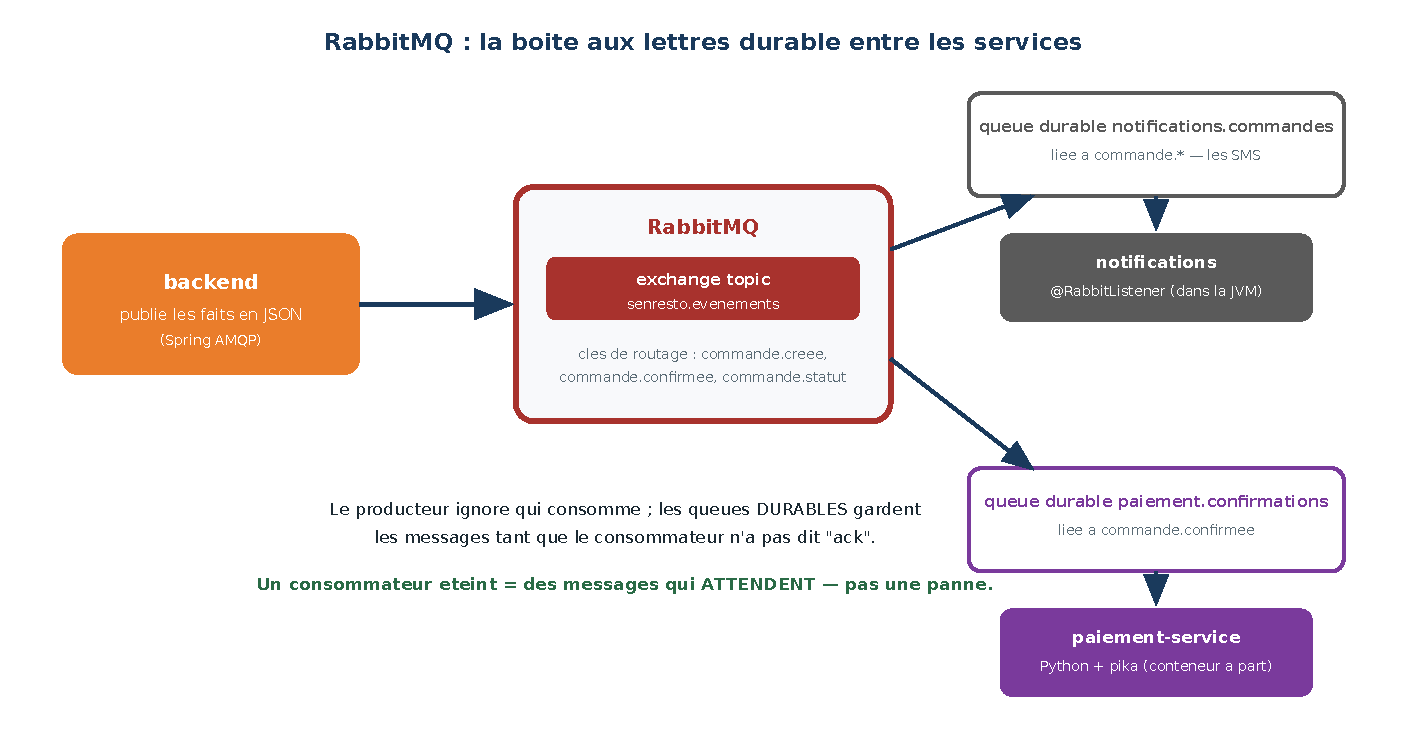
\includegraphics[width=0.86\textwidth]{figs/figN_broker.pdf}
\caption{La cible : le broker au centre, deux queues durables, deux langages.}
\end{figure}

% =====================================================================
\section{Etape 1 --- Le broker et le pont}
% =====================================================================

\begin{collabox}
\textbf{L'Huissier} pilote compose et RabbitMQ. \textbf{Le Doyen} pilote le
pont AMQP. \textbf{Le Rédacteur} prend possession de l'UI de gestion.
\end{collabox}

\subsection{RabbitMQ dans l'orchestre}

Dans \texttt{docker-compose.yml} :

\begin{lstlisting}[language=bash]
  rabbitmq:
    image: rabbitmq:3-management
    ports: ["5672:5672", "15672:15672"]   # AMQP + UI de gestion
\end{lstlisting}

Le backend en dépend (\texttt{depends\_on}) et reçoit la variable
\texttt{SPRING\_RABBITMQ\_HOST} valant \texttt{rabbitmq}. L'interface de
gestion est sur le port \texttt{15672} (guest / guest) : votre poste
d'observation pour toute la séance.

\subsection{Le pont : les faits partent en JSON}

Dépendance \texttt{spring-boot-starter-amqp}, puis deux briques dans un
nouveau module \texttt{evenements/} (ou dans \texttt{commandes/interne} :
discutez, c'est une ligne d'ADR) :

\begin{lstlisting}[language=java]
@Configuration
class ConfigurationAmqp {
    @Bean TopicExchange evenements() {
        return new TopicExchange("senresto.evenements", true, false);
    }
    @Bean Jackson2JsonMessageConverter json() {
        return new Jackson2JsonMessageConverter();   // records -> JSON
    }
}
\end{lstlisting}

\begin{lstlisting}[language=java]
@Component
class PontAmqp {
    private final RabbitTemplate rabbit;
    PontAmqp(RabbitTemplate rabbit) { this.rabbit = rabbit; }

    @EventListener
    void quandCreee(CommandeCreee evt)         { publier("commande.creee", evt); }
    @EventListener
    void quandConfirmee(CommandeConfirmee evt) { publier("commande.confirmee", evt); }
    @EventListener
    void quandStatut(CommandeStatutChangee evt){ publier("commande.statut", evt); }

    private void publier(String cle, Object evt) {
        rabbit.convertAndSend("senresto.evenements", cle, evt);
    }
}
\end{lstlisting}

\begin{pointcle}
\texttt{CommandeMetier} n'a pas bougé d'une ligne : il publie ses faits
comme au Lab 3. Le pont \emph{écoute et réexpédie} --- les frontières du
modulith paient une dernière fois.
\end{pointcle}

\begin{warningbox}
\textbf{Le réflexe du Lab 4, réappliqué :} annotez
\texttt{ConfigurationAmqp} et \texttt{PontAmqp} de
\texttt{@Profile("amqp")} --- sans broker (CI, \texttt{mvnw test}), le
pont n'existe pas et les 10 juges restent verts ; compose active
\texttt{amqp}. Même geste pour notifications à l'étape 2 : l'ancien
\texttt{@EventListener} reste sous \texttt{@Profile("!amqp")} (le chemin
historique du Strangler), le nouveau \texttt{@RabbitListener} vit sous
\texttt{@Profile("amqp")}.
\end{warningbox}

\begin{todobox}
Compose à 5 conteneurs ; dans l'UI, créez une queue temporaire liée à
\texttt{commande.\#}, passez une commande : \textbf{regardez le JSON
arriver}. 10 juges toujours verts (le pont ne casse rien).
\end{todobox}

\begin{tagbox}
\begin{center}\texttt{git tag lab5-etape1 \&\& git push origin lab5-etape1}\end{center}
\end{tagbox}

% =====================================================================
\section{Etape 2 --- Les consommateurs}
% =====================================================================

\begin{collabox}
\textbf{Le Notaire} migre notifications. \textbf{L'Appariteur} pilote la
deuxième extraction : \texttt{paiement-service} en Python.
\end{collabox}

\subsection{Notifications : la queue durable}

Déclarez la queue et son binding (beans \texttt{Queue} et
\texttt{Binding}, motif \texttt{commande.*}), puis remplacez les
écouteurs internes d'\texttt{EcouteurNotifications} par :

\begin{lstlisting}[language=java]
@RabbitListener(queues = "notifications.commandes")
void surEvenement(Map<String, Object> evt,
        @Header("amqp_receivedRoutingKey") String cle) {
    switch (cle) {
        case "commande.creee" -> sms.envoyerSms(/* MEMES textes qu'avant */);
        // confirmee, statut : meme principe
    }
}
\end{lstlisting}

\subsection{Paiement demenage --- sans facade}

Supprimez le module \texttt{paiement} du monolithe (il déménage —
c'est la mort par famine du figuier : plus rien ne l'appelle), et créez
\texttt{paiement-service/} (conteneur Python) :

\begin{lstlisting}[language=python]
# paiement-service/main.py -- pika, ~40 lignes
import json, os, pika

params = pika.ConnectionParameters(host=os.environ.get("RABBITMQ_HOST", "localhost"))
connexion = pika.BlockingConnection(params)
canal = connexion.channel()
canal.exchange_declare("senresto.evenements", "topic", durable=True)
canal.queue_declare("paiement.confirmations", durable=True)
canal.queue_bind("paiement.confirmations", "senresto.evenements",
                 "commande.confirmee")

deja_traites = set()          # l'idempotence, version simple

def sur_message(canal, methode, proprietes, corps):
    evt = json.loads(corps)
    if evt["commandeId"] in deja_traites:
        print(f"[PAIEMENT] {evt['numero']} deja traite, ignore", flush=True)
    else:
        deja_traites.add(evt["commandeId"])
        print(f"[PAIEMENT] Encaissement mobile money simule : "
              f"{evt['montantTotal']} FCFA pour la commande {evt['numero']}",
              flush=True)
    canal.basic_ack(methode.delivery_tag)     # l'ack APRES le traitement

canal.basic_consume("paiement.confirmations", sur_message)
print("[PAIEMENT] paiement-service en ecoute...", flush=True)
canal.start_consuming()
\end{lstlisting}

\begin{pointcle}
Comparez au Lab 4 : cette extraction n'a exigé \textbf{ni interface, ni
profils, ni timeouts, ni 503}. Personne n'attend la réponse du paiement :
l'extraction asynchrone est radicalement moins chère. C'est LA leçon du
cours : \emph{le coût d'une frontière dépend de la nature de l'échange qui
la traverse}.
\end{pointcle}

\begin{todobox}
6 conteneurs ; parcours complet : les \texttt{[SMS]} sortent du backend
(via la queue), le \texttt{[PAIEMENT]} sort de \textbf{son} conteneur
(\texttt{docker compose logs -f paiement-service}). 10 juges verts.
\end{todobox}

\begin{tagbox}
\begin{center}\texttt{git tag lab5-etape2 \&\& git push origin lab5-etape2}\end{center}
\end{tagbox}

% =====================================================================
\section{Etape finale --- La demonstration miroir}
% =====================================================================

\begin{collabox}
\textbf{Tous ensemble}, au vidéoprojecteur --- c'est la scène finale du
semestre, elle se joue en cinq actes.
\end{collabox}

\begin{figure}[h]
\centering
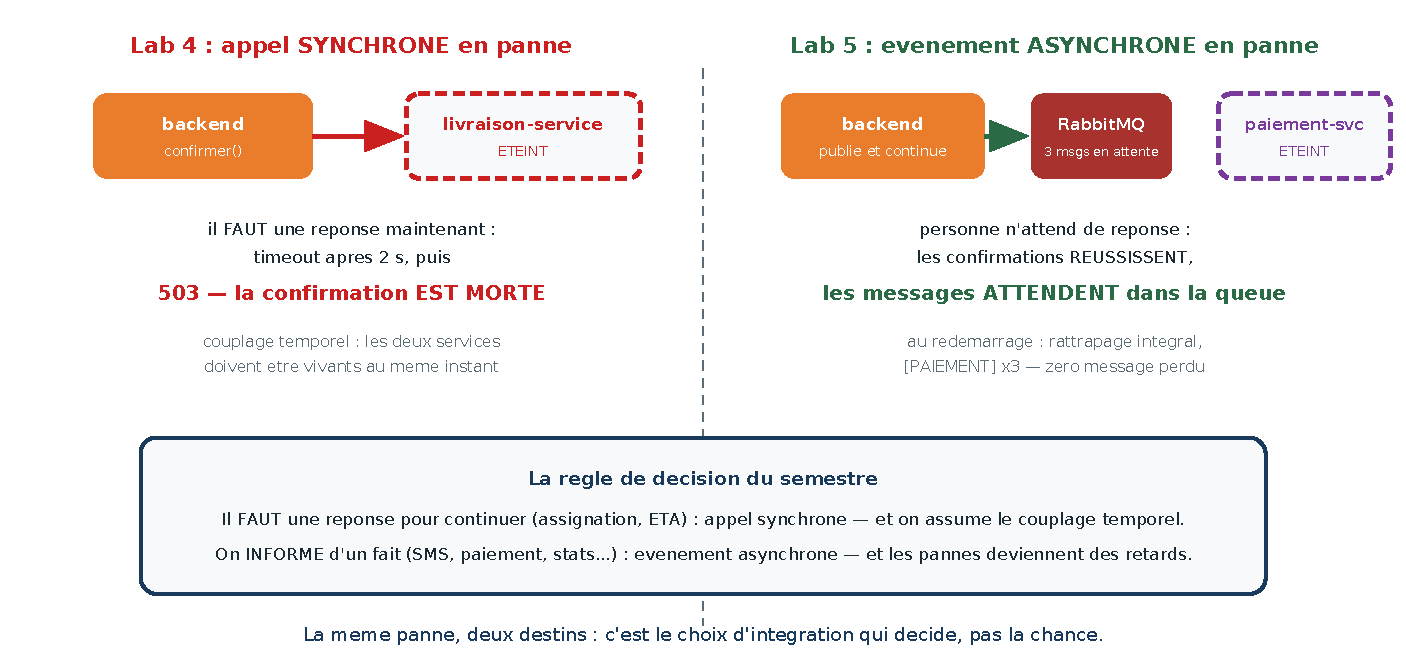
\includegraphics[width=0.92\textwidth]{figs/figO_miroir.pdf}
\caption{La même panne, deux destins.}
\end{figure}

\begin{enumerate}[nosep]
  \item \texttt{docker compose stop paiement-service} --- le paiement est mort.
  \item Passez et confirmez \textbf{trois} commandes : tout réussit,
        \textbf{aucun 503} --- comparez au Lab 4, même geste, autre destin.
  \item L'UI de gestion : la queue \texttt{paiement.confirmations} affiche
        \textbf{3 messages prêts}, qui attendent.
  \item \texttt{docker compose start paiement-service} : dans ses logs, le
        \textbf{rattrapage} --- \texttt{[PAIEMENT]} $\times$3, dans l'ordre.
  \item Bonus idempotence : dans l'UI, re-publiez à la main un des messages
        (onglet \emph{Publish message}) : \texttt{deja traite, ignore}.
        Un webhook Wave rejoué ne doit \emph{jamais} encaisser deux fois.
\end{enumerate}

\begin{warningbox}
Constatez aussi ce que l'asynchrone \textbf{ne répare pas} : l'assignation
du livreur reste synchrone (il \emph{faut} l'ETA dans la réponse), et les
blessures « statut manuel » et « état évaporé » restent ouvertes ---
mais vous savez désormais \emph{exactement} comment un événement
\texttt{course.terminee} publié par le service Python les refermerait.
C'est votre premier chantier d'après-cours.
\end{warningbox}

\begin{tagbox}
Démo des 5 actes réalisée et notée :
\begin{center}\texttt{git tag lab5-final \&\& git push origin lab5-final}\end{center}
\end{tagbox}

% =====================================================================
\section{ADR, livrable et cloture}
% =====================================================================

L'\textbf{Architecte du jour} signe l'\textbf{ADR n\textsuperscript{o}5 : « Synchrone ou
asynchrone ? »}, dans \texttt{docs/adr/} : le tableau de
\emph{toutes} les intégrations de SénResto (assignation, SMS, paiement,
positions, statuts) avec, pour chacune, le mode choisi et la justification
--- il faut une réponse, ou l'on informe d'un fait ?

\begin{center}
\small
\begin{tabular}{p{0.62\textwidth}p{0.28\textwidth}}
\toprule
\textbf{Critère} & \textbf{Vérification} \\
\midrule
4 tags ; 10 juges verts & \texttt{git tag}, \texttt{mvnw clean test} \\
Le JSON observé dans l'UI ; queues durables liées & UI 15672 \\
\texttt{[PAIEMENT]} depuis son conteneur & \texttt{compose logs} \\
La démo miroir : 3 attendus, 3 rattrapés, 0 perdu & notes + capture \\
Idempotence prouvée (message rejoué ignoré) & logs \\
ADR n\textsuperscript{o}5 : le tableau complet des intégrations & \texttt{docs/adr/} \\
\bottomrule
\end{tabular}
\end{center}

\vspace{0.5em}
\noindent\textbf{Clôture.} En cinq séances, la même application est passée
du God controller au système distribué polyglotte et résilient --- sous
tests à chaque pas, chaque décision tracée. Gardez ce dépôt : c'est votre
portfolio d'architecte.

\vspace{1em}
\begin{center}
\textit{Fin du Lab 5 --- et du fil rouge SénResto --- Dr. El Hadji Bassirou TOURE --- DMI/FST/UCAD}
\end{center}

\end{document}
